
% utf-8 ru, unix eolns
\documentclass[12pt,a4paper,oneside]{extarticle}
    \righthyphenmin=2 %минимально переносится 2 символа %%%
    \sloppy

% Рукопись оформлена в соответствии с правилами оформления 
% электронной версии авторского оригинала, 
% принятыми в Издательстве МГТУ им. Н.Э. Баумана.

\usepackage{geometry} % А4, примерно 28-31 строк(а) на странице 
    \geometry{paper=a4paper}
    \geometry{includehead=false} % Нет верх. колонтитула
    \geometry{includefoot=true}  % Есть номер страницы
    \geometry{bindingoffset=0mm} % Переплет    : 0  мм
    \geometry{top=20mm}          % Поле верхнее: 20 мм
    \geometry{bottom=25mm}       % Поле нижнее : 25 мм 
    \geometry{left=25mm}         % Поле левое  : 25 мм
    \geometry{right=25mm}        % Поле правое : 25 мм
    \geometry{headsep=10mm}  % От края до верх. колонтитула: 10 мм
    \geometry{footskip=20mm} % От края до нижн. колонтитула: 20 мм 

\usepackage{cmap}
\usepackage[T2A]{fontenc} 
\usepackage[utf8x]{inputenc}
\usepackage[english,russian]{babel}
\usepackage{misccorr}

\usepackage{amsmath}
\usepackage{amsfonts}
\usepackage{amssymb}

%\usepackage{cm-super} %человеческий рендер русских шрифтов

\setlength{\parindent}{1.25cm}  % Абзацный отступ: 1,25 см
\usepackage{indentfirst}        % 1-й абзац имеет отступ

\usepackage{setspace}   

\onehalfspacing % Полуторный интервал между строками

\makeatletter
\renewcommand{\@oddfoot }{\hfil\thepage\hfil} % Номер стр.
\renewcommand{\@evenfoot}{\hfil\thepage\hfil} % Номер стр.
\renewcommand{\@oddhead }{} % Нет верх. колонтитула
\renewcommand{\@evenhead}{} % Нет верх. колонтитула
\makeatother

\usepackage{fancyvrb}


\usepackage[pdftex]{graphicx}  % поддержка картинок для пдф
\graphicspath{ {./pictures/} }
\usepackage{rotating}
%\DeclareGraphicsExtensions{.jpg,.png}




\renewcommand{\labelenumi}{\theenumi.} %меняет вид нумерованного списка

\usepackage{perpage} %нумерация сносок 
\MakePerPage{footnote}

\usepackage[all]{xy} %поддержка графов

\usepackage{listings} %листинги
\renewcommand{\lstlistingname}{Листинг}
\lstset{
  basicstyle=\tiny,
  breaklines=true
  }


\usepackage{url}


\usepackage{tikz} %для рисования графиков
\usepackage{pgfplots}

\usepackage{gensymb}

\usepackage{ccaption}%изменяет подпись к рисунку
\makeatletter 
\renewcommand{\fnum@figure}[1]{Рисунок~\thefigure~---~\sffamily}
\makeatother

\begin{document}
\pgfplotsset{compat=1.8}

\thispagestyle{empty}
\newpage
{
\centering


\textbf{
МОСКОВСКИЙ ГОСУДАРСТВЕННЫЙ ТЕХНИЧЕСКИЙ УНИВЕРСИТЕТ ИМЕНИ Н. Э. БАУМАНА \\
Факультет информатики и систем управления \\
Кафедра теоретической информатики и компьютерных технологий}
\bigskip
\bigskip
\bigskip
\bigskip
\bigskip
\bigskip
\bigskip

\vfill


Лабораторная работа №3 \\
по курсу <<Современные вычислительные методы>>

\bigskip

{\large <<Аналитическое построение уравнения границы сложной области>>}
\bigskip

\vfill



\hfill\parbox{4cm} {
Выполнил:\\
студент ИУ9-111 \hfill \\
Выборнов А. И.\hfill \medskip\\
Руководитель:\\
Басараб М.А.\hfill
}


\vspace{\fill}

Москва \number\year
\clearpage
}

\clearpage


\section{Постановка задачи}
    Для области, изображенной на схеме, построить нормализованное уравнение границы Г в неявной форме:
    $$F (x, y) = 0$$
    Визуализировать линии уровня функции $z = f (x, y)$.

    Построить «функцию склейки» $U(x,y)$, принимающую значения -1 и 1 на участках границы Г$_-$ и Г$_+$, расположенных слева и справа от вертикальной оси симметрии области соответственно. Визуализировать линии уровня функции $z = U (x, y)$.
    Область имеет следующий вид:
    \begin{figure}[ht!]
        \centering
        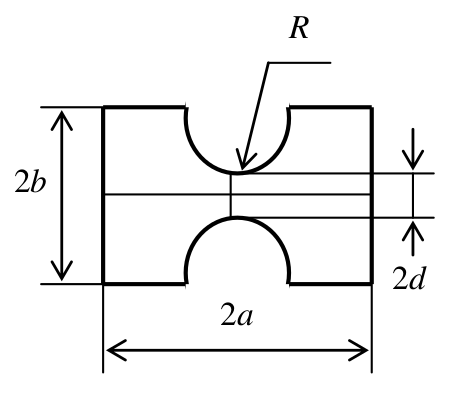
\includegraphics[scale=0.5]{p1.png}
        \label{pic:p1}
    \end{figure}

    Заданы следующие параметры:
    $$a = 4.5, b=2.5,d=1.$$

\section{Решение}
    Будем рассматривать исходную фигуру как прямоугольник со сторонами $2b$ и $2a$ из которого были вырезаны две окружности с радиусом $R=b-d$.

    Прямоугольник зададим границами $z_1$ и $z_2$:
    $$z_1 = \dfrac{a^2-x^2}{2a},$$
    $$z_2 = \dfrac{b^2-y^2}{2b}.$$

    А две окружности радиуса $R$ с центрами в точках $(0,b)$ и $(0, -b)$ зададим границами $z_3$ и $z_4$:
    $$z_3 = \dfrac{R^2-x^2-(y-b)^2}{2R},$$
    $$z_4 = \dfrac{R^2-x^2-(y+b)^2}{2R}.$$

    По найденным границам посторим уравнение границы $F$:
    $$F = (z_1 \wedge z_2) \wedge \lnot (z_3 \vee z_4). $$
    Визуализация функции $F(x,y)$ изображена на рисунке~\ref{pic:f1}.

    \begin{figure}[ht!]
        \centering
        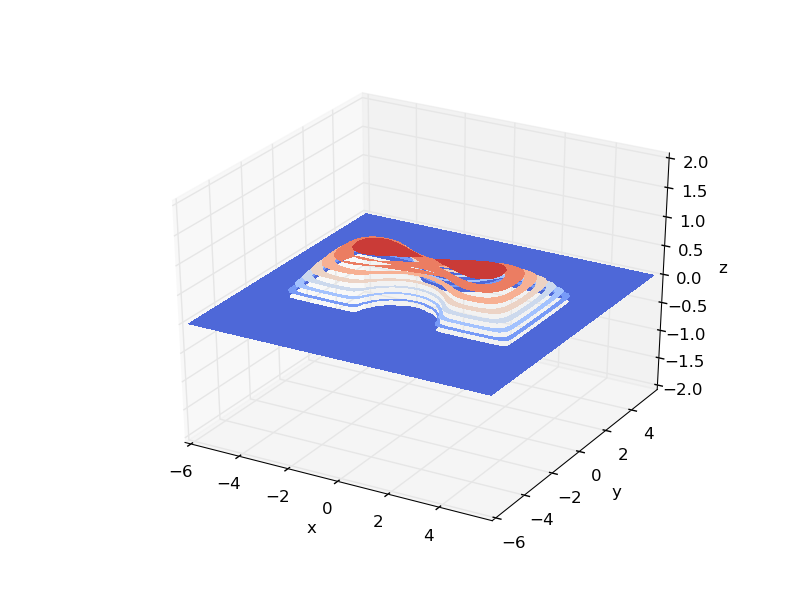
\includegraphics[scale=0.8]{figure_1.png}
        \caption{Визуализация линий уровня функции $F(x,y)$ в полуплоскости $z > 0$}
        \label{pic:f1}
    \end{figure}

    Построим «функцию склейки» $U$, следующий образом:
    \begin{gather}
        U(x,y) = 
        \begin{cases}
            sign(x),~ F(x,y) < 0; \nonumber \\
            0, ~ F(x,y) \ge 0.
        \end{cases}
    \end{gather}
    Визуализация функции $U(x,y)$ изображена на рисунке~\ref{pic:f2}.

    \begin{figure}[ht!]
        \centering
        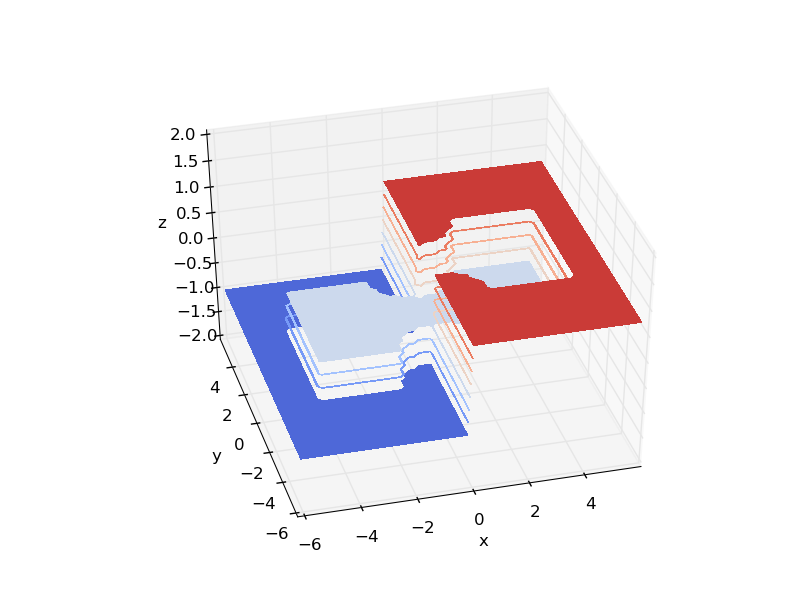
\includegraphics[scale=0.8]{figure_2.png}
        \caption{Визуализация линий уровня функции $U(x,y)$}
        \label{pic:f2}
    \end{figure}

\end{document}

